\chapter{Аутентификация и Авторизация}\label{chap:auth}

Аутентификация и авторизация~--- две тесно связанные, но в то же время
различные концепции. Тогда как первая имеет дело с идентификацией пользователя,
вторая определяет, что пользователю позволено делать. К сожалению, поскольку
для обоих терминов часто используется сокращение <<auth>>, эти концепции часто
объединяются.

Yesod имеет встроенную поддержку для нескольких сторонних систем
аутентификации, таких как OpenID, BrowserID и OAuth. Это внешние системы,
которым ваше приложение доверяет удостоверение личности пользователя. Также
есть поддержка более привычных способов аутентификации, таких как имя
пользователя и пароль или адрес почты и пароль. Первый способ гарантирует
простоту как для пользователей (нет неоходимости запоминать новые пароли), так
и для разработчиков (нет нужды иметь дело со всей архитектурой безопасности), в
то время как второй даёт разработчику больший контроль.

Для авторизации мы можем воспользоваться преимуществами REST и типобезопасными
URL, чтобы создать простую и декларативную систему. К тому же, поскольку весь
код авторизации написан на Haskell, в вашем распоряжении будет вся гибкость
языка.

В этой главе мы рассмотрим, как настроить <<auth>> в Yesod, и обсудим некоторые
плюсы и минусы различных вариантов аутентификации.

\section{Обзор}


Пакет \footnotehref{http://hackage.haskell.org/package/yesod-auth}{yesod-auth}
предоставляет унифицированный интерфейс для различных плагинов аутентификации.
Единственное, что требуется от этих плагинов, так это чтобы они
идентифицировали пользователя по какой-нибудь уникальной строке. В OpenID, к
примеру, это может быть фактическое значение OpenID. В BrowserID это адрес
электронной почты. Для HashDB (которая использует базу данных хешированных
паролей) это имя пользователя.

Каждый плагин аутентификации предоставляет свою собственную систему для входа
на сайт, будь то передача токенов с внешнего сайта или же форма входа с вводом
адреса почты и пароля. После успешного входа плагин устанавливает значение в
пользовательской сессии, определяющее его \lstinline'AuthId'. Значением этого
\lstinline'AuthId' обычно является Persistent ID из таблицы, используемой для
отслеживания пользователей.

Есть несколько функций, позволяющих получить пользовательский
\lstinline'AuthId', наиболее используемыми из которых являются
\lstinline'maybeAuthId', \lstinline'requireAuthId', \lstinline'maybeAuth' и
\lstinline'requireAuth'. Версии с \lstinline'require' перенаправляют на
страницу входа, если пользователь ещё не вошёл, а те функции, что не
оканчиваются на \lstinline'Id', возвращают два значения: ID в таблице и
значение сущности.

Поскольку хранение \lstinline'AuthId' построено на сессиях, то применимы все их
правила. В частности, данные сохраняются в зашифрованном, подписанном HMAC
куки, которое автоматически устаревает после определённого, задаваемого в
конфигурации, периода неактивности. Кроме того, поскольку не существует
серверной составляющей сессий, то при выходе из системы просто удаляются данные
из куки этой сессии, и если пользователь повторно использует старое значение
куки, то сессия будет всё ещё считаться действительной.

\begin{remark}
    Есть планы добавления серверной составляющей сессий, которая позволила бы
    форсировать выход.
\end{remark}

С другой стороны, авторизация контролируется несколькими методами внутри класса
типов \lstinline'Yesod'. Эти методы запускаются для каждого запроса, чтобы
определить~--- разрешить пользователю доступ, запретить его, или же потребовать
от пользователя войти на сайт. По умолчанию эти методы разрешают доступ для
каждого запроса. В качестве альтернативы вы можете реализовать авторизацию
способом, подходящим для конкретного случая, вызывая \lstinline'requireAuth' и
подобные ей функции в индивидуальных функциях-обработчиках, хотя это и
отрицательно отразится на преимуществах декларативной системы авторизации.

\section{Аутентифицируй меня}

Давайте сразу рассмотрим пример с аутентификацией.

\includecode{14/authentication.hs}

Начнём с объявлений маршрутов. Сперва объявляем наш стандартный маршрут
\lstinline'HomeR', а затем определяем подсайт для аутентификации. Помните, что
ему нужны четыре параметра: путь к подсайту, имя маршрута, имя подсайта и
функция для получения значения подсайта. Другими словами, судя по строке

\begin{lstlisting}
/auth AuthR Auth getAuth
\end{lstlisting}

Нам нужно иметь функцию \lstinline'getAuth :: MyAuthSite -> Auth'. Пока мы не
напишем эту функцию сами,
\footnotehref{http://hackage.haskell.org/package/yesod-auth}{\lstinline'yesod-auth'}
предоставляет её автоматически. Для других подсайтов (к примеру, со
статическими файлами) мы указываем настройки конфигурации в значении подсайта,
и поэтому нам нужно определять функцию \lstinline'get'. Для auth-подсайта мы
указываем эти настройки в отдельном классе типов~\lstinline'YesodAuth'.

\begin{remark}
    Почему бы не использовать значение подсайта? Существует достаточно много
    настроек, которые мы бы хотели передать auth-подсайту, и делать это из типа
    записи (record type) было бы неудобно. Также, поскольку мы хотим иметь
    ассоциируемый тип \lstinline'AuthId', использование класса типов будет
    более естественным.

    С другой стороны, почему бы не использовать класс типов для всех подсайтов?
    У такого подхода есть минус: вы сможете иметь только один экземпляр класса
    на сайт, не позволяя раздавать различные группы статичных файлов с
    различных маршрутов. Также, если мы хотим загружать данные во время
    иницииализации приложения, значение подсайта подойдёт лучше.
\end{remark}

Так что же именно входит в экземпляр класса \lstinline'YesodAuth'? Шесть
объявлений являются обязательными:

\begin{itemize}
    \item Ассоциированный тип \lstinline'AuthId'. Это то значение, которое
        \lstinline'yesod-auth' будет возвращать вам, когда вы будете
        запрашивать, вошёл ли пользователь (через \lstinline'maybeAuthId'
        или~\lstinline'requireAuthId'). В нашем случае мы просто используем
        \lstinline'Text' для сохранения необработанного идентификатора. Как вы
        скоро увидите, в нашем случае это адрес электронной почты.

    \item \lstinline'getAuthId' получает текущий \lstinline'AuthId' из типа
        данных \lstinline'Creds' (credentials~--- учётные данные). Этот тип
        содержит три фрагмента информации: используемый способ аутентификации
        (в нашем случае browserid или googleemail), текущий идентификатор и
        ассоциированный список с различной дополнительной информацией.

    \item \lstinline'loginDest' возвращает маршрут, на который перенаправляется
        пользователь после успешного входа.

    \item Аналогичным образом \lstinline'logoutDest' возвращает маршрут, на
        который происходит перенаправление после выхода.

    \item \lstinline'authPlugins'~--- это список используемых способов
        аутентификации. В нашем примере мы используем BrowserID, который входит
        через систему Mozilla BrowserID, и Google Email, который
        аутентифицирует почтовый адрес пользователя, используя его учётную
        запись Google. Что хорошо в этих двух способах, так это то, что:

    \begin{itemize}
        \item Они не требуют установки, в отличие от Facebook или OAuth,
            которые требуют задания учётных данных.

        \item Они используют в качестве идентификатора привычный людям адрес
            электронной почты, в отличие от OpenID, который использует URL.
    \end{itemize}

    \item \lstinline'authHttpManager' получает менеджер HTTP-соединений из
        основного типа. Это позволяет системам аутентификации, которые
        используют HTTP-соединения (то есть почти всем сторонним системам
        входа), использовать эти соединения повторно, избегая затрат на
        установку нового TCP-соединения для каждого запроса.
\end{itemize}

Кроме описанных шести доступны и другие методы для управления поведением
системы аутентификации, например, видом страницы для входа. За информацией
обращайтесь к
\footnotehref{http:\\hackage.haskell.org/package/yesod-auth-1.2.5.2/docs/Yesod-Auth.html\#t:YesodAuth}{описанию API}.

Наш обработчик \lstinline'HomeR' содержит ссылки на страницы входа и выхода,
которые отображаются в зависимости от того, вошёл пользователь на сайт или нет.
Обратите внимание, как мы конструируем эти ссылки на подсайт: первым идёт имя
маршрута подсайта (\lstinline'AuthR'), следом маршрут в подсайте
(\lstinline'LoginR' и \lstinline'LogoutR').

Иллюстрации ниже показывают процесс входа со стороны пользователя.

\begin{figure}[h!]
  \centering
  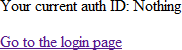
\includegraphics[width=0.4\textwidth]{14-initial-screen.png}
  \caption{Начальная загрузка страницы}
\end{figure}

\begin{figure}[h!]
  \centering
  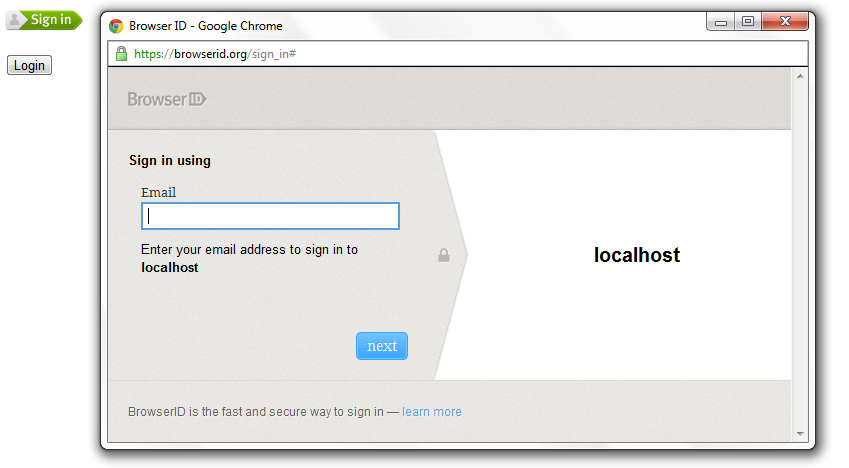
\includegraphics[width=1\textwidth]{14-login-with-browserid.png}
  \caption{Экран входа с помощью BrowserID}
\end{figure}

\begin{figure}[h!]
  \centering
  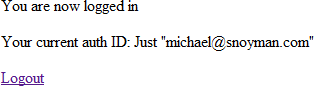
\includegraphics[width=0.6\textwidth]{14-after-login.png}
  \caption{Домашняя страница после входа}
\end{figure}

\section{Электронная почта}

Для большинства случаев будет достаточно аутентификации по адресу электронной
почты, осуществляемой сторонним сервисом. Но иногда вам может понадобиться,
чтобы пользователи использовали для вашего сайта пароль. Сгенерированый сайт не
включает эту функциональность, так как:

\begin{itemize}
    \item Чтобы безопасно использовать пароли, надо использовать SSL. Многие
        пользователи не предоставляют доступ к сайту по SSL.

    \item Несмотря на то, что система аутентификации по адресу электронной
        почты должным образом хранит пароли (с использованием хеширования и
        <<соли>>), скомпрометированная база данных всё равно может быть
        проблемой. Помните: мы не делаем никаких предположений о том, что
        пользователи Yesod используют безопасные методы развёртывания.

    \item Вам нужна работающая система для отправки электронной почты. Многие
        веб-серверы в наши дни не имеют достаточных средств для защиты от спама
        по сравнению с теми, что используют почтовые сервера.

    \begin{remark}
        Пример ниже использует системную программу для отправки писем~---
        sendmail. Если вы хотите избежать хлопот, работая с серверами
        электронной почты самостоятельно, вы можете использовать Amazon SES.
        Есть пакет
        \footnotehref{http://hackage.haskell.org/package/mime-mail-ses}{mime-mail-ses},
        который предоставляет альтернативу использованию sendmail. Этот подход
        мы используем на сайте Haskellers.com.
    \end{remark}
\end{itemize}

Но если предположить, что вы можете удовлетворить эти требования и хотите иметь
вход по паролю именно для вашего сайта, то Yesod может предложить встроенную
систему аутентификации. Для её использования от вас потребуется немного больше
кода, ведь будет необходимо безопасно сохранять пароли в базе данных и
отправлять пользователю почтовые сообщения (верификация учётной записи,
восстановление пароля, и т.д.).

Давайте посмотрим на сайт, предоставляющий аутентификацию по адресу электронной
почты и паролю и хранящий пароли в Persistent базе данных SQLite.

\includecode{14/email-authentication.hs}

\section{Авторизация}

Как только вы получили возможность аутентифицировать пользователей, вы можете
использовать их учётные данные для \emph{авторизации} дальнейших запросов.
Авторизация в Yesod проста и декларативна: в большинстве случаев необходимо
всего лишь добавить методы \lstinline'authRoute' и \lstinline'isAuthorized' в
ваш экземпляр класса типов \lstinline'Yesod'. Давайте рассмотрим пример:

\includecode{14/authorization.hs}

\lstinline'authRoute' должен быть вашей страницей входа, почти всегда это будет
\lstinline'AuthR LoginR'. Функция \lstinline'isAuthorized' имеет два параметра:
запрашиваемый маршрут, и является или нет запрос запросом на запись. На самом
деле вы можете переопределить, что именно является запросом на запись,
используя метод \lstinline'isWriteRequest', но реализация <<из коробки>>
следует принципам RESTful: все запросы, кроме \lstinline'GET',
\lstinline'HEAD', \lstinline'OPTIONS' или \lstinline'TRACE'~--- это запросы на
запись.

В теле \lstinline'isAuthorized' вы можете исполнять любой
\lstinline'Handler'-код, какой только захотите, что очень удобно. Это означает,
что вы можете:

\begin{itemize}
    \item обращаться к файловой системе (обычный ввод/вывод);

    \item делать запросы к базе данных;

    \item получать любые параметры сессии или запроса.
\end{itemize}

Используя эти техники, вы можете разработать настолько сложную систему
авторизации, насколько захотите, или даже привязаться к уже существующей
системе, используемой в вашей организации.

\section{Выводы}

Эта глава рассматривает основы настройки аутентификации пользователей, а также
то, как встроенные функции авторизации предоставляют пользователям простой и
декларативный механизм. Хотя это и сложные концепции со многими подходами,
Yesod предоставляет все необходимые строительные блоки для построения системы
аутентификации и авторизации, соответствующей вашим требованиям.
